\chapter{Endoscopic Ultrasound (EUS)}
\label{ch:endoscopic_ultrasound}

% Chapter-opening illustrated modality infographic.
\begin{center}
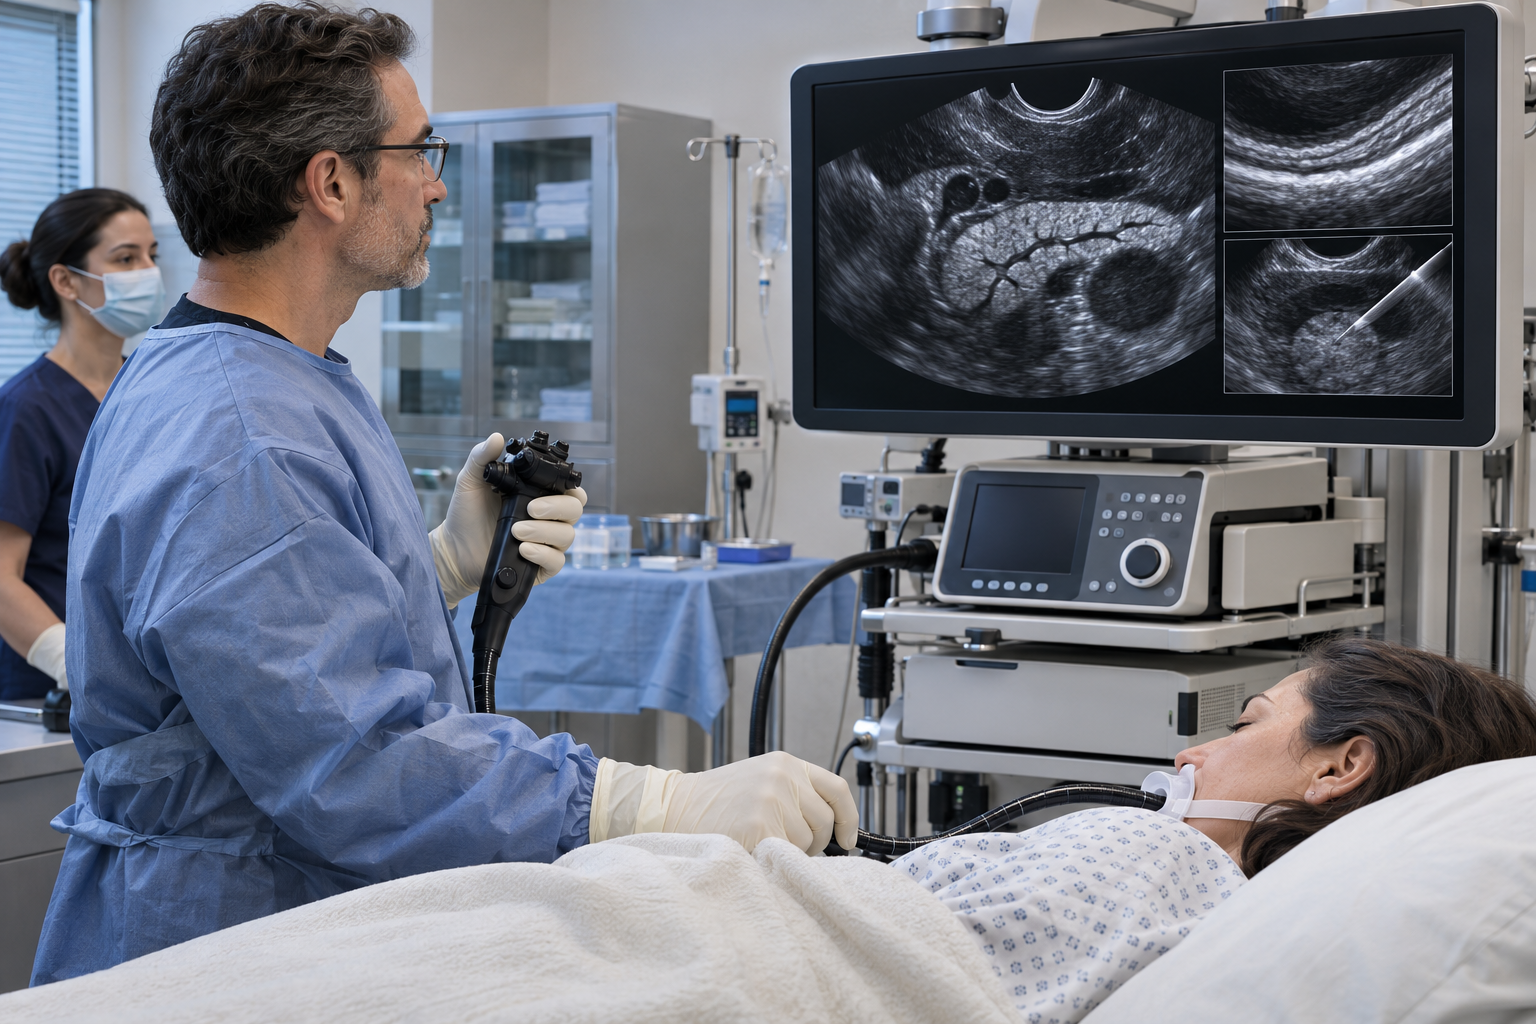
\includegraphics[width=\textwidth,keepaspectratio]{modalities/infographics/endoscopic_imaging_eus_realistic.png}
\end{center}
\begin{center}\footnotesize EUS places an ultrasound transducer close to the gastrointestinal wall and nearby organs, supporting detailed imaging and guided sampling. AI-generated illustration; ultrasound and biopsy panels are schematic.\end{center}

\section{Overview}
Endoscopic ultrasound (EUS), also known as endosonography, combines flexible endoscopy with high-frequency ultrasound imaging. An ultrasound transducer mounted at the tip of an endoscope visualizes the gastrointestinal wall and adjacent organs, blood vessels, lymph nodes and pathological structures.

Unlike conventional transabdominal ultrasound, EUS positions the transducer close to the target, reducing interference from abdominal fat, bowel gas and overlying anatomical structures. EUS is especially useful for pancreatic lesions, gastrointestinal subepithelial lesions, local staging of gastrointestinal malignancies, small biliary stones, image-guided tissue acquisition, lymph-node assessment and selected minimally invasive therapies.

\section{Where endoscopic ultrasound is used}

\subsection{Pancreatic diseases}
\begin{enumerate}[leftmargin=*,itemsep=0.45em,topsep=0.4em]
\item \textbf{Acinar cell carcinoma.} Useful imaging findings include: Solid heterogeneous pancreatic mass.
\item \textbf{Acute pancreatitis.} Useful imaging findings include: Variable, nonspecific parenchymal changes; EUS is generally supplementary and may investigate an occult biliary cause after the acute episode.
\item \textbf{Annular pancreas.} Useful imaging findings include: Pancreatic tissue surrounding the duodenum.
\item \textbf{Autoimmune pancreatitis.} Useful imaging findings include: Diffuse or focal hypoechoic pancreatic enlargement.
\item \textbf{Chronic pancreatitis.} Useful imaging findings include: Hyperechoic strands, lobularity, calcifications and ductal abnormalities.
\item \textbf{Early chronic pancreatitis.} Useful imaging findings include: Subtle, nonspecific parenchymal and ductal abnormalities; interpret with clinical findings and other imaging.
\item \textbf{Fatty pancreas.} Useful imaging findings include: Increased parenchymal echogenicity.
\item \textbf{Gastrinoma.} Useful imaging findings include: Hypoechoic neuroendocrine lesion.
\item \textbf{Glucagonoma.} Useful imaging findings include: Solid pancreatic mass with variable vascularity.
\item \textbf{Insulinoma.} Useful imaging findings include: Small, well-circumscribed hypoechoic lesion.
\item \textbf{Pancreas divisum.} Useful imaging findings include: Abnormal pancreatic ductal configuration.
\item \textbf{Pancreatic adenocarcinoma.} Useful imaging findings include: Irregular hypoechoic solid mass, sometimes with ductal obstruction.
\item \textbf{Pancreatic atrophy.} Useful imaging findings include: Reduced parenchymal volume.
\item \textbf{Pancreatic calcification.} Useful imaging findings include: Hyperechoic foci with acoustic shadowing.
\item \textbf{Pancreatic duct obstruction.} Useful imaging findings include: Upstream pancreatic duct dilatation.
\item \textbf{Pancreatic duct stone.} Useful imaging findings include: Echogenic intraductal focus with posterior shadowing.
\item \textbf{Pancreatic duct stricture.} Useful imaging findings include: Focal ductal narrowing with possible upstream dilatation.
\item \textbf{Pancreatic lipoma.} Useful imaging findings include: Well-defined hyperechoic lesion.
\item \textbf{Pancreatic lymphoma.} Useful imaging findings include: Hypoechoic pancreatic mass or diffuse enlargement.
\item \textbf{Pancreatic metastases.} Useful imaging findings include: Discrete solid lesions with variable echogenicity.
\item \textbf{Pancreatic necrosis.} Useful imaging findings include: Heterogeneous areas; nonenhancement is assessed with contrast-enhanced EUS, not conventional B-mode imaging.
\item \textbf{Pancreatic neuroendocrine tumor.} Useful imaging findings include: Well-defined, frequently hypoechoic and hypervascular mass.
\item \textbf{Solid pseudopapillary neoplasm.} Useful imaging findings include: Encapsulated mass with solid and cystic components.
\item \textbf{VIPoma.} Useful imaging findings include: Well-defined solid pancreatic lesion.
\end{enumerate}

\subsection{Pancreatic cystic lesions}
\begin{enumerate}[leftmargin=*,itemsep=0.45em,topsep=0.4em]
\item \textbf{Acute necrotic collection.} Useful imaging findings include: Heterogeneous fluid and necrotic material without a mature wall.
\item \textbf{Acute peripancreatic fluid collection.} Useful imaging findings include: Fluid collection without a mature encapsulating wall.
\item \textbf{Branch-duct IPMN.} Useful imaging findings include: Cystic lesion communicating with a pancreatic duct branch.
\item \textbf{Cystic degeneration of pancreatic carcinoma.} Useful imaging findings include: Irregular cystic mass with solid components.
\item \textbf{Cystic pancreatic neuroendocrine tumor.} Useful imaging findings include: Cystic lesion with an enhancing solid component.
\item \textbf{Main-duct IPMN.} Useful imaging findings include: Dilatation of the main pancreatic duct.
\item \textbf{Mixed-type IPMN.} Useful imaging findings include: Combined main-duct and branch-duct abnormalities.
\item \textbf{Mucinous cystic neoplasm.} Useful imaging findings include: Macrocystic lesion with septations and possible mural nodules.
\item \textbf{Pancreatic duplication cyst.} Useful imaging findings include: Cystic structure with characteristic layered wall.
\item \textbf{Pancreatic lymphangioma.} Useful imaging findings include: Multiloculated cystic lesion.
\item \textbf{Pancreatic lymphoepithelial cyst.} Useful imaging findings include: Cystic lesion with variable internal echogenicity.
\item \textbf{Pancreatic pseudocyst.} Useful imaging findings include: Fluid-filled collection with a defined wall.
\item \textbf{Pancreatic retention cyst.} Useful imaging findings include: Simple cystic lesion associated with ductal obstruction.
\item \textbf{Serous cystadenoma.} Useful imaging findings include: Microcystic or honeycomb-like architecture, sometimes with a central scar.
\item \textbf{Walled-off pancreatic necrosis.} Useful imaging findings include: Encapsulated collection containing heterogeneous necrotic debris.
\end{enumerate}
EUS morphology alone cannot reliably differentiate all pancreatic cystic neoplasms. Cyst-fluid analysis, cytology, molecular testing and MRI/MRCP may provide complementary information. EUS-guided sampling is selective and is most useful when the result is likely to change management.

\subsection{Gallbladder and biliary tract diseases}
\begin{enumerate}[leftmargin=*,itemsep=0.45em,topsep=0.4em]
\item \textbf{Acute cholecystitis.} Useful imaging findings include: Gallbladder wall thickening and surrounding inflammatory changes.
\item \textbf{Benign biliary stricture.} Useful imaging findings include: Relatively smooth focal bile duct narrowing.
\item \textbf{Biliary ascariasis.} Useful imaging findings include: Linear echogenic intraductal structure.
\item \textbf{Biliary microlithiasis.} Useful imaging findings include: Small echogenic intraductal structures.
\item \textbf{Biliary obstruction.} Useful imaging findings include: Proximal biliary dilatation and possible obstructing lesion.
\item \textbf{Biliary sludge.} Useful imaging findings include: Low-level intraluminal echoes, generally without shadowing.
\item \textbf{Choledochal cyst.} Useful imaging findings include: Abnormal cystic dilatation of the biliary tract.
\item \textbf{Choledocholithiasis.} Useful imaging findings include: Echogenic stone within the common bile duct.
\item \textbf{Cholelithiasis.} Useful imaging findings include: Hyperechoic gallstones with posterior acoustic shadowing.
\item \textbf{Cholesterol polyp.} Useful imaging findings include: Small echogenic polypoid lesion.
\item \textbf{Chronic cholecystitis.} Useful imaging findings include: Gallbladder wall thickening and possible calculi.
\item \textbf{Common bile duct dilatation.} Useful imaging findings include: Increased bile duct diameter.
\item \textbf{Distal cholangiocarcinoma.} Useful imaging findings include: Hypoechoic mass or irregular bile duct wall thickening.
\item \textbf{Gallbladder adenoma.} Useful imaging findings include: Solid polypoid lesion with variable echogenicity.
\item \textbf{Gallbladder adenomyomatosis.} Useful imaging findings include: Intramural cystic spaces and comet-tail artifacts.
\item \textbf{Gallbladder carcinoma.} Useful imaging findings include: Irregular wall thickening or infiltrative mass.
\item \textbf{Gallbladder microlithiasis.} Useful imaging findings include: Small echogenic particulate structures.
\item \textbf{Hilar cholangiocarcinoma.} Useful imaging findings include: Irregular hilar biliary lesion, when accessible.
\item \textbf{IgG4-related sclerosing cholangitis.} Useful imaging findings include: Possible bile duct wall thickening; EUS findings are nonspecific and do not establish the diagnosis.
\item \textbf{Malignant biliary stricture.} Useful imaging findings include: Irregular narrowing with abnormal surrounding tissue.
\item \textbf{Mirizzi syndrome.} Useful imaging findings include: Impacted gallstone associated with extrinsic biliary compression.
\item \textbf{Primary sclerosing cholangitis.} Useful imaging findings include: Possible ductal wall thickening; EUS findings are nonspecific and do not establish the diagnosis.
\end{enumerate}
EUS can assess accessible bile duct segments and investigate focal abnormalities, but it does not establish primary sclerosing or IgG4-related cholangitis. Diagnosis requires clinical and laboratory correlation with cholangiographic imaging, typically MRCP, and other testing as indicated.

\subsection{Ampullary and periampullary diseases}
\begin{enumerate}[leftmargin=*,itemsep=0.45em,topsep=0.4em]
\item \textbf{Ampullary adenoma.} Useful imaging findings include: Localized ampullary soft-tissue lesion.
\item \textbf{Ampullary carcinoma.} Useful imaging findings include: Irregular hypoechoic ampullary mass.
\item \textbf{Ampullary inflammatory enlargement.} Useful imaging findings include: Thickened or enlarged ampullary tissue.
\item \textbf{Ampullary neuroendocrine tumor.} Useful imaging findings include: Small solid hypoechoic lesion.
\item \textbf{Ampullary obstruction.} Useful imaging findings include: Ampullary abnormality with upstream ductal dilatation.
\item \textbf{Intraductal extension of ampullary tumor.} Useful imaging findings include: Extension of abnormal tissue into pancreatic or bile ducts.
\item \textbf{Periampullary carcinoma.} Useful imaging findings include: Mass involving the ampullary region or adjacent structures.
\item \textbf{Periampullary duodenal diverticulum.} Useful imaging findings include: Outpouching adjacent to the ampulla.
\end{enumerate}

\subsection{Esophageal diseases}
\begin{enumerate}[leftmargin=*,itemsep=0.45em,topsep=0.4em]
\item \textbf{Esophageal adenocarcinoma.} Useful imaging findings include: Irregular mural thickening with possible transmural invasion.
\item \textbf{Esophageal duplication cyst.} Useful imaging findings include: Anechoic or hypoechoic cystic lesion with a layered wall.
\item \textbf{Esophageal gastrointestinal stromal tumor.} Useful imaging findings include: Hypoechoic lesion commonly arising from muscularis propria.
\item \textbf{Esophageal granular cell tumor.} Useful imaging findings include: Small hypoechoic subepithelial lesion.
\item \textbf{Esophageal leiomyoma.} Useful imaging findings include: Well-defined hypoechoic lesion arising from a muscular layer.
\item \textbf{Esophageal lipoma.} Useful imaging findings include: Hyperechoic submucosal lesion.
\item \textbf{Esophageal lymphoma.} Useful imaging findings include: Abnormal wall thickening with possible lymphadenopathy.
\item \textbf{Esophageal schwannoma.} Useful imaging findings include: Solid hypoechoic subepithelial lesion.
\item \textbf{Esophageal squamous cell carcinoma.} Useful imaging findings include: Hypoechoic lesion disrupting normal esophageal wall layers.
\item \textbf{Esophageal varices.} Useful imaging findings include: Anechoic tubular vascular structures with Doppler flow.
\item \textbf{Esophageal wall infiltration.} Useful imaging findings include: Loss or disruption of normal wall architecture.
\item \textbf{Extrinsic esophageal compression.} Useful imaging findings include: External structure compressing an otherwise preserved esophageal wall.
\item \textbf{Paraesophageal varices.} Useful imaging findings include: Dilated vascular channels outside the esophageal wall.
\end{enumerate}

\subsection{Gastric diseases}
\begin{enumerate}[leftmargin=*,itemsep=0.45em,topsep=0.4em]
\item \textbf{Advanced gastric carcinoma.} Useful imaging findings include: Deep mural invasion and possible adjacent organ involvement.
\item \textbf{Early gastric carcinoma.} Useful imaging findings include: Localized superficial wall abnormality.
\item \textbf{Ectopic pancreas.} Useful imaging findings include: Heterogeneous subepithelial lesion, sometimes containing duct-like structures.
\item \textbf{Gastric adenocarcinoma.} Useful imaging findings include: Irregular hypoechoic wall thickening and layer disruption.
\item \textbf{Gastric amyloidosis.} Useful imaging findings include: Variable thickening of gastric wall layers.
\item \textbf{Gastric duplication cyst.} Useful imaging findings include: Cystic lesion with layered wall.
\item \textbf{Gastric extrinsic compression.} Useful imaging findings include: External mass compressing the gastric wall.
\item \textbf{Gastric gastrointestinal stromal tumor (GIST).} GIST is a mesenchymal tumor that often arises from the muscularis propria; EUS assesses layer of origin, margins, and risk features. Useful imaging findings include: Hypoechoic mass commonly arising from muscularis propria.
\item \textbf{Gastric glomus tumor.} Useful imaging findings include: Hypoechoic or heterogeneous vascular mass.
\item \textbf{Gastric inflammatory fibroid polyp.} Useful imaging findings include: Hypoechoic lesion involving mucosal or submucosal layers.
\item \textbf{Gastric leiomyoma.} Useful imaging findings include: Homogeneous hypoechoic muscular lesion.
\item \textbf{Gastric linitis plastica.} Useful imaging findings include: Diffuse infiltrative wall thickening and loss of normal stratification.
\item \textbf{Gastric lipoma.} Useful imaging findings include: Homogeneous hyperechoic submucosal lesion.
\item \textbf{Gastric lymphoma.} Useful imaging findings include: Diffuse or localized hypoechoic wall thickening.
\item \textbf{Gastric MALT lymphoma.} Useful imaging findings include: Variable mucosal and submucosal thickening.
\item \textbf{Gastric metastases.} Useful imaging findings include: Focal or diffuse mural infiltration.
\item \textbf{Gastric neuroendocrine tumor.} Useful imaging findings include: Small hypoechoic mucosal or submucosal lesion.
\item \textbf{Gastric schwannoma.} Useful imaging findings include: Well-defined hypoechoic subepithelial lesion.
\item \textbf{Gastric varices.} Useful imaging findings include: Tortuous anechoic vascular channels with Doppler flow.
\item \textbf{M\'en\'etrier disease.} Useful imaging findings include: Predominantly mucosal thickening.
\end{enumerate}

\subsection{Duodenal and small intestinal diseases}
\begin{enumerate}[leftmargin=*,itemsep=0.45em,topsep=0.4em]
\item \textbf{Brunner gland hamartoma.} Useful imaging findings include: Variable heterogeneous or cystic submucosal lesion.
\item \textbf{Duodenal adenocarcinoma.} Useful imaging findings include: Irregular hypoechoic mural lesion.
\item \textbf{Duodenal duplication cyst.} Useful imaging findings include: Cystic lesion with layered wall.
\item \textbf{Duodenal endometriosis.} Useful imaging findings include: Hypoechoic infiltrative mural lesion in selected cases.
\item \textbf{Duodenal GIST.} Useful imaging findings include: Solid hypoechoic lesion arising from muscularis propria.
\item \textbf{Duodenal lipoma.} Useful imaging findings include: Hyperechoic submucosal mass.
\item \textbf{Duodenal lymphoma.} Useful imaging findings include: Abnormal mural thickening.
\item \textbf{Duodenal neuroendocrine tumor.} Useful imaging findings include: Small hypoechoic subepithelial lesion.
\item \textbf{Duodenal wall invasion by pancreatic carcinoma.} Useful imaging findings include: Disruption of wall layers by an adjacent mass.
\item \textbf{Small intestinal subepithelial lesion.} Useful imaging findings include: Lesion characterized by wall-layer origin and echogenicity.
\end{enumerate}
Conventional EUS principally accesses the upper gastrointestinal tract and selected lower regions. Most of the jejunum and ileum cannot be routinely reached.

\subsection{Colorectal and anorectal diseases}
\begin{enumerate}[leftmargin=*,itemsep=0.45em,topsep=0.4em]
\item \textbf{Anal carcinoma.} Useful imaging findings include: Irregular infiltrative hypoechoic lesion.
\item \textbf{Anal sphincter atrophy.} Useful imaging findings include: Reduced muscle thickness.
\item \textbf{Anal sphincter injury.} Useful imaging findings include: Discontinuity of sphincter musculature.
\item \textbf{Early rectal carcinoma.} Useful imaging findings include: Localized superficial tumor infiltration.
\item \textbf{Intersphincteric abscess.} Useful imaging findings include: Collection between internal and external sphincters.
\item \textbf{Locally advanced rectal carcinoma.} Useful imaging findings include: Extension beyond muscularis propria.
\item \textbf{Perianal abscess.} Useful imaging findings include: Hypoechoic or heterogeneous fluid collection.
\item \textbf{Perianal fistula.} Useful imaging findings include: Hypoechoic fistulous tract.
\item \textbf{Perirectal lymphadenopathy.} Useful imaging findings include: Enlarged lymph nodes adjacent to the rectum.
\item \textbf{Rectal adenocarcinoma.} Useful imaging findings include: Hypoechoic mural mass disrupting normal wall layers.
\item \textbf{Rectal duplication cyst.} Useful imaging findings include: Cystic lesion adjacent to or within the rectal wall.
\item \textbf{Rectal endometriosis.} Useful imaging findings include: Hypoechoic infiltrative lesion frequently involving muscularis propria.
\item \textbf{Rectal GIST.} Useful imaging findings include: Hypoechoic muscularis propria lesion.
\item \textbf{Rectal leiomyoma.} Useful imaging findings include: Homogeneous hypoechoic muscular lesion.
\item \textbf{Rectal lipoma.} Useful imaging findings include: Hyperechoic submucosal lesion.
\item \textbf{Rectal lymphoma.} Useful imaging findings include: Abnormal mural thickening.
\item \textbf{Rectal neuroendocrine tumor.} Useful imaging findings include: Small hypoechoic submucosal lesion.
\item \textbf{Rectal varices.} Useful imaging findings include: Dilated submucosal vascular channels.
\end{enumerate}
Some of these conditions are evaluated using dedicated endorectal ultrasound (ERUS) or endoanal ultrasound (EAUS), rather than a conventional gastrointestinal echoendoscope.

\subsection{Hepatic diseases}
\begin{enumerate}[leftmargin=*,itemsep=0.45em,topsep=0.4em]
\item \textbf{Focal nodular hyperplasia.} Useful imaging findings include: Solid lesion with variable echogenicity.
\item \textbf{Granulomatous liver disease.} Useful imaging findings include: Variable focal or diffuse abnormalities.
\item \textbf{Hepatic abscess.} Useful imaging findings include: Complex fluid collection with internal echoes.
\item \textbf{Hepatic adenoma.} Useful imaging findings include: Solid lesion with variable internal architecture.
\item \textbf{Hepatic hemangioma.} Useful imaging findings include: Frequently well-defined hyperechoic lesion.
\item \textbf{Hepatic lymphoma.} Useful imaging findings include: Hypoechoic focal lesions or infiltrative abnormalities.
\item \textbf{Hepatic metastases.} Useful imaging findings include: Focal lesions with variable echogenicity.
\item \textbf{Hepatic steatosis.} Useful imaging findings include: Increased hepatic echogenicity.
\item \textbf{Hepatocellular carcinoma.} Useful imaging findings include: Focal solid lesion with variable vascular enhancement.
\item \textbf{Intrahepatic cholangiocarcinoma.} Useful imaging findings include: Irregular hypoechoic hepatic mass.
\item \textbf{Liver cirrhosis.} Useful imaging findings include: Coarse echotexture and irregular surface where visible.
\item \textbf{Simple hepatic cyst.} Useful imaging findings include: Anechoic lesion with posterior acoustic enhancement.
\end{enumerate}
EUS visualizes selected hepatic segments, particularly portions of the left lobe. It does not replace comprehensive liver imaging with transabdominal ultrasound, CT or MRI.

\subsection{Lymphatic and lymph node diseases}
\begin{enumerate}[leftmargin=*,itemsep=0.45em,topsep=0.4em]
\item \textbf{Celiac lymphadenopathy.} Useful imaging findings include: Enlarged lymph nodes around celiac vessels.
\item \textbf{Hodgkin lymphoma.} Useful imaging findings include: Enlarged hypoechoic lymph nodes.
\item \textbf{Mediastinal lymphadenopathy.} Useful imaging findings include: Enlarged nodes accessible through the esophageal wall.
\item \textbf{Metastatic lymphadenopathy.} Useful imaging findings include: Rounded hypoechoic nodes with possible sharp margins.
\item \textbf{Necrotic lymphadenopathy.} Useful imaging findings include: Heterogeneous nodes containing hypoechoic or cystic regions.
\item \textbf{Non-Hodgkin lymphoma.} Useful imaging findings include: Multiple enlarged or conglomerate lymph nodes.
\item \textbf{Peripancreatic lymphadenopathy.} Useful imaging findings include: Enlarged nodes adjacent to the pancreas.
\item \textbf{Periportal lymphadenopathy.} Useful imaging findings include: Enlarged nodes around portal structures.
\item \textbf{Reactive lymphadenopathy.} Useful imaging findings include: Variable nodal enlargement, sometimes with preserved architecture.
\item \textbf{Retroperitoneal lymphadenopathy.} Useful imaging findings include: Enlarged nodes within accessible retroperitoneal regions.
\item \textbf{Sarcoidosis.} Useful imaging findings include: Multiple enlarged mediastinal or abdominal lymph nodes.
\item \textbf{Tuberculous lymphadenitis.} Useful imaging findings include: Enlarged nodes with possible necrosis.
\end{enumerate}
Lymph-node morphology alone cannot reliably distinguish infection, inflammation and malignancy. EUS-guided tissue acquisition can improve diagnostic specificity.

\subsection{Mediastinal and thoracic diseases}
\begin{enumerate}[leftmargin=*,itemsep=0.45em,topsep=0.4em]
\item \textbf{Bronchogenic cyst.} Useful imaging findings include: Well-defined cystic mediastinal lesion.
\item \textbf{Centrally located lung carcinoma.} Useful imaging findings include: Solid pulmonary lesion adjacent to the esophagus.
\item \textbf{Mediastinal duplication cyst.} Useful imaging findings include: Cystic lesion with characteristic wall architecture.
\item \textbf{Mediastinal lymphoma.} Useful imaging findings include: Enlarged hypoechoic lymph nodes or confluent mass.
\item \textbf{Mediastinal metastases.} Useful imaging findings include: Solid masses or abnormal lymph nodes.
\item \textbf{Mediastinal sarcoidosis.} Useful imaging findings include: Multiple enlarged lymph nodes.
\item \textbf{Mediastinal schwannoma.} Useful imaging findings include: Well-defined hypoechoic solid mass.
\item \textbf{Mediastinal tuberculosis.} Useful imaging findings include: Lymphadenopathy with variable necrotic components.
\item \textbf{Pleural effusion.} Useful imaging findings include: Anechoic fluid within the pleural space.
\item \textbf{Posterior mediastinal tumor.} Useful imaging findings include: Solid lesion adjacent to the esophagus.
\end{enumerate}
Endobronchial ultrasound (EBUS) is related but distinct; it accesses tracheobronchial and mediastinal structures through the respiratory tract.

\subsection{Adrenal and retroperitoneal diseases}
\begin{enumerate}[leftmargin=*,itemsep=0.45em,topsep=0.4em]
\item \textbf{Adrenal adenoma.} Useful imaging findings include: Discrete adrenal lesion with variable echogenicity.
\item \textbf{Adrenal cyst.} Useful imaging findings include: Anechoic adrenal lesion.
\item \textbf{Adrenal hemorrhage.} Useful imaging findings include: Heterogeneous adrenal enlargement.
\item \textbf{Adrenal metastasis.} Useful imaging findings include: Enlarged or irregular adrenal mass.
\item \textbf{Adrenal myelolipoma.} Useful imaging findings include: Frequently echogenic heterogeneous lesion.
\item \textbf{Adrenocortical carcinoma.} Useful imaging findings include: Large heterogeneous adrenal lesion.
\item \textbf{Pheochromocytoma.} Useful imaging findings include: Solid adrenal lesion with variable vascularity.
\item \textbf{Retroperitoneal cyst.} Useful imaging findings include: Cystic lesion adjacent to accessible gastrointestinal structures.
\item \textbf{Retroperitoneal lymphoma.} Useful imaging findings include: Hypoechoic masses or enlarged lymph nodes.
\item \textbf{Retroperitoneal sarcoma.} Useful imaging findings include: Large heterogeneous soft-tissue mass.
\end{enumerate}
The left adrenal gland is generally more accessible than the right. Suspected pheochromocytoma should be investigated biochemically before invasive tissue sampling is considered.

\subsection{Vascular diseases and abnormalities}
\begin{enumerate}[leftmargin=*,itemsep=0.45em,topsep=0.4em]
\item \textbf{Esophageal varices.} Useful imaging findings include: Dilated submucosal venous structures.
\item \textbf{Gastric varices.} Useful imaging findings include: Dilated vascular channels within or around the gastric wall.
\item \textbf{Pancreatic tumor vascular invasion.} Useful imaging findings include: Abnormal tumor-vessel interface, encasement or luminal distortion.
\item \textbf{Perigastric collateral circulation.} Useful imaging findings include: Multiple abnormal venous channels.
\item \textbf{Portal cavernous transformation.} Useful imaging findings include: Multiple collateral vascular channels.
\item \textbf{Portal hypertension.} Useful imaging findings include: Dilated portosystemic collateral vessels.
\item \textbf{Portal vein thrombosis.} Useful imaging findings include: Intraluminal material and reduced or absent Doppler flow.
\item \textbf{Splenic artery aneurysm.} Useful imaging findings include: Focal arterial dilatation with Doppler flow.
\item \textbf{Splenic vein thrombosis.} Useful imaging findings include: Abnormal intraluminal echoes and impaired venous flow.
\item \textbf{Superior mesenteric vein thrombosis.} Useful imaging findings include: Venous filling abnormality and reduced flow.
\item \textbf{Tumor thrombus.} Useful imaging findings include: Intravascular tissue with possible internal vascularity.
\item \textbf{Visceral artery pseudoaneurysm.} Useful imaging findings include: Vascular sac with characteristic Doppler flow.
\end{enumerate}

\subsection{Other abdominal and extraluminal conditions}
\begin{enumerate}[leftmargin=*,itemsep=0.45em,topsep=0.4em]
\item \textbf{Abdominal duplication cyst.} Useful imaging findings include: Cystic lesion with characteristic wall layering.
\item \textbf{Ascites.} Useful imaging findings include: Anechoic fluid surrounding abdominal structures.
\item \textbf{Extraluminal gastrointestinal tumor.} Useful imaging findings include: Solid mass adjacent to the gastrointestinal tract.
\item \textbf{Intra-abdominal abscess.} Useful imaging findings include: Complex fluid-containing lesion.
\item \textbf{Intra-abdominal hematoma.} Useful imaging findings include: Heterogeneous collection with evolving echogenicity.
\item \textbf{Lymphocele.} Useful imaging findings include: Localized cystic fluid collection.
\item \textbf{Malignant ascites.} Useful imaging findings include: Fluid with possible associated peritoneal nodules.
\item \textbf{Omental metastases.} Useful imaging findings include: Abnormal nodular soft-tissue deposits.
\item \textbf{Peritoneal carcinomatosis.} Useful imaging findings include: Irregular peritoneal nodules or thickening.
\item \textbf{Postoperative pancreatic fluid collection.} Useful imaging findings include: Localized fluid collection near pancreatic structures.
\end{enumerate}



\subsection{Summary of catalogue}
\begin{tabular}{@{}p{0.70\textwidth}r@{}}
\toprule
\textbf{Disease category} & \textbf{Entries} \\
\midrule
Adrenal and retroperitoneal diseases & 10 \\
Ampullary and periampullary diseases & 8 \\
Colorectal and anorectal diseases & 18 \\
Duodenal and small intestinal diseases & 10 \\
Esophageal diseases & 13 \\
Gallbladder and biliary tract diseases & 22 \\
Gastric diseases & 20 \\
Hepatic diseases & 12 \\
Lymphatic and lymph node diseases & 12 \\
Mediastinal and thoracic diseases & 10 \\
Other abdominal and extraluminal conditions & 10 \\
Pancreatic cystic lesions & 15 \\
Pancreatic diseases & 24 \\
Total & 196 \\
Vascular diseases and abnormalities & 12 \\
\bottomrule
\end{tabular}

\subsection{Types of endoscopic ultrasound}
\begin{longtable}{@{}p{0.38\textwidth}p{0.56\textwidth}@{}}
\toprule
\textbf{EUS technique} & \textbf{Primary application} \\
\midrule
\endfirsthead
\toprule
\textbf{EUS technique} & \textbf{Primary application} \\
\midrule
\endhead
B-mode EUS & Grayscale structural imaging \\
Color Doppler EUS & Blood flow visualization \\
Contrast-enhanced EUS & Tissue vascularity and perfusion assessment \\
Contrast-enhanced harmonic EUS & Microvascular enhancement characterization \\
Endoanal ultrasound (EAUS) & Anal sphincter and perianal anatomy \\
Endorectal ultrasound (ERUS) & Rectal wall and surrounding tissue evaluation \\
EUS shear-wave elastography & Quantitative tissue stiffness estimation \\
EUS strain elastography & Relative tissue stiffness assessment \\
High-frequency miniprobe EUS & Superficial gastrointestinal wall characterization \\
Intraductal ultrasound (IDUS) & High-resolution pancreatic and biliary duct imaging \\
Linear-array EUS & Anatomical imaging and image-guided interventions \\
Power Doppler EUS & Detection of low-velocity blood flow \\
Radial EUS & Circumferential cross-sectional anatomical imaging \\
Spectral Doppler EUS & Quantitative blood flow assessment \\
Three-dimensional EUS & Volumetric reconstruction \\
\bottomrule
\end{longtable}

\subsection{Normal gastrointestinal wall architecture}
One distinctive capability of EUS is visualization of the individual sonographic layers of the gastrointestinal wall.

\begin{longtable}{@{}p{0.15\textwidth}p{0.24\textwidth}p{0.55\textwidth}@{}}
\toprule
\textbf{Layer} & \textbf{Echogenicity} & \textbf{Corresponding anatomical structure} \\
\midrule
\endfirsthead
\toprule
\textbf{Layer} & \textbf{Echogenicity} & \textbf{Corresponding anatomical structure} \\
\midrule
\endhead
Layer 1 & Hyperechoic & Superficial mucosa and luminal interface \\
Layer 2 & Hypoechoic & Deep mucosa \\
Layer 3 & Hyperechoic & Submucosa \\
Layer 4 & Hypoechoic & Muscularis propria \\
Layer 5 & Hyperechoic & Serosa, adventitia and surrounding interface \\
\bottomrule
\end{longtable}
These are the conventional five sonographic layers. Higher-frequency imaging may resolve additional layers.

\subsection{Differentiation of subepithelial lesions}
\begin{longtable}{@{}p{0.28\textwidth}p{0.27\textwidth}p{0.39\textwidth}@{}}
\toprule
\textbf{Lesion} & \textbf{Typical layer of origin} & \textbf{Echogenicity} \\
\midrule
\endfirsthead
\toprule
Duplication cyst & Variable & Anechoic or hypoechoic \\
\midrule
\endhead
Ectopic pancreas & Variable, often third or fourth layer & Heterogeneous \\
GIST & Usually fourth layer & Hypoechoic \\
Granular cell tumor & Second or third layer & Hypoechoic \\
Leiomyoma & Second or fourth layer & Hypoechoic \\
\textbf{Lesion} & \textbf{Typical layer of origin} & \textbf{Echogenicity} \\
Lipoma & Third layer & Hyperechoic \\
Neuroendocrine tumor & Second or third layer & Hypoechoic \\
Schwannoma & Usually fourth layer & Hypoechoic \\
Varices & Third layer or extramural & Anechoic with Doppler flow \\
\bottomrule
\end{longtable}

\subsection{Contrast-enhanced EUS}
Contrast-enhanced EUS uses intravenously administered microbubble contrast agents to characterize tissue perfusion and microvascular architecture.

\begin{longtable}{@{}p{0.40\textwidth}p{0.54\textwidth}@{}}
\toprule
\textbf{Disease or condition} & \textbf{Typical enhancement pattern} \\
\midrule
\endfirsthead
\toprule
\textbf{Disease or condition} & \textbf{Typical enhancement pattern} \\
\midrule
\endhead
Autoimmune pancreatitis & Variable homogeneous enhancement \\
Chronic inflammatory pancreatic mass & Variable, sometimes isoenhancement \\
Gallbladder carcinoma & Irregular or heterogeneous vascular enhancement \\
Gallbladder sludge & Absent enhancement \\
GIST & Variable enhancement, sometimes with irregular intratumoral vessels \\
Intracystic mucus or debris & Generally absent internal enhancement \\
Necrotic lymph node & Nonenhancing central region \\
Pancreatic cyst mural nodule & Enhancement of viable nodular tissue \\
Pancreatic ductal adenocarcinoma & Hypoenhancement relative to surrounding pancreas \\
Pancreatic necrosis & Absent enhancement in necrotic tissue \\
Pancreatic neuroendocrine tumor & Frequently hyperenhancement \\
Pancreatic pseudocyst & No enhancement of internal fluid \\
\bottomrule
\end{longtable}
Enhancement patterns overlap among diseases and should not be treated as definitive histological classifications.

\subsection{EUS elastography}
EUS elastography estimates tissue mechanical properties. Diseased tissues may differ in stiffness because of fibrosis, inflammation, cellular proliferation or extracellular matrix changes.

\begin{longtable}{@{}p{0.40\textwidth}p{0.54\textwidth}@{}}
\toprule
\textbf{Disease or condition} & \textbf{Typical elastographic finding} \\
\midrule
\endfirsthead
\toprule
\textbf{Disease or condition} & \textbf{Typical elastographic finding} \\
\midrule
\endhead
Autoimmune pancreatitis & Increased or heterogeneous stiffness \\
Chronic pancreatitis & Increased stiffness associated with fibrosis \\
Hepatic fibrosis & Increased hepatic stiffness \\
Malignant lymphadenopathy & Frequently increased stiffness \\
Pancreatic adenocarcinoma & Frequently increased stiffness \\
Pancreatic fibrosis & Increased parenchymal stiffness \\
Pancreatic neuroendocrine tumor & Variable stiffness \\
Reactive lymphadenopathy & Variable, often relatively softer tissue \\
\bottomrule
\end{longtable}
Elastography is supplementary and cannot reliably distinguish malignancy from inflammation in every case.

\subsection{EUS-guided diagnostic and therapeutic procedures}
\begin{longtable}{@{}p{0.48\textwidth}p{0.46\textwidth}@{}}
\toprule
\textbf{Procedure} & \textbf{Clinical application} \\
\midrule
\endfirsthead
\toprule
\textbf{Procedure} & \textbf{Clinical application} \\
\midrule
\endhead
EUS-guided adrenal biopsy & Selected adrenal mass characterization \\
EUS-guided biliary drainage & Management of biliary obstruction \\
EUS-guided celiac plexus block & Selected pancreatic pain management \\
EUS-guided celiac plexus neurolysis & Selected pancreatic cancer pain management \\
EUS-guided choledochoduodenostomy & Creation of a bile duct drainage pathway \\
EUS-guided cyst ablation & Specialized or investigational pancreatic cyst treatment \\
EUS-guided fiducial placement & Radiation therapy targeting \\
EUS-guided fine-needle aspiration (FNA) & Cytological sampling \\
EUS-guided fine-needle biopsy (FNB) & Histological tissue acquisition \\
EUS-guided gallbladder drainage & Management of selected high-risk cholecystitis patients \\
EUS-guided gastroenterostomy & Selected gastric outlet obstruction \\
EUS-guided glue injection & Selected gastric variceal obliteration \\
EUS-guided hepaticogastrostomy & Drainage of intrahepatic bile ducts \\
EUS-guided liver biopsy & Selected hepatic tissue sampling \\
EUS-guided lymph node biopsy & Investigation of lymphadenopathy \\
EUS-guided pancreatic cyst aspiration & Selected cyst-fluid analysis when results are likely to change management \\
EUS-guided pancreatic duct drainage & Selected pancreatic duct obstruction \\
EUS-guided pelvic abscess drainage & Selected accessible pelvic collections \\
EUS-guided portal pressure measurement & Emerging portal hypertension assessment \\
EUS-guided pseudocyst drainage & Drainage of symptomatic pancreatic pseudocysts \\
EUS-guided radiofrequency ablation & Selected pancreatic lesions; specialized or emerging \\
EUS-guided tumor injection & Investigational localized therapies \\
EUS-guided vascular coil embolization & Selected gastric varices \\
EUS-guided walled-off necrosis drainage & Management of selected pancreatic necrotic collections \\
\bottomrule
\end{longtable}

\subsection{Physical characteristics of EUS}
\begin{longtable}{@{}p{0.39\textwidth}p{0.55\textwidth}@{}}
\toprule
\textbf{Parameter} & \textbf{Typical characteristics} \\
\midrule
\endfirsthead
\toprule
\textbf{Parameter} & \textbf{Typical characteristics} \\
\midrule
\endhead
Contrast mechanism & Acoustic impedance differences \\
Conventional operating frequency & Approximately 5--12 MHz \\
Functional imaging & Doppler and contrast enhancement \\
High-frequency miniprobe & Approximately 12--30 MHz \\
Imaging dimensions & Two-dimensional, dynamic and selected three-dimensional acquisitions \\
Invasiveness & Minimally invasive endoscopic examination \\
Ionizing radiation & None \\
Mechanical characterization & Elastography \\
Penetration depth & Frequency- and tissue-dependent \\
Physical mechanism & Acoustic pulse--echo imaging \\
Spatial resolution & Submillimeter under favorable conditions \\
Tissue acquisition & FNA and FNB \\
Transducer position & Inside gastrointestinal lumen \\
\bottomrule
\end{longtable}

Acoustic wavelength is given by:
\[
\lambda=\frac{c}{f}
\]
where $c$ is the speed of sound in tissue and $f$ is ultrasound frequency. Assuming a soft-tissue sound velocity of approximately 1,540 m/s:

\begin{longtable}{@{}p{0.45\textwidth}p{0.49\textwidth}@{}}
\toprule
\textbf{Transducer frequency} & \textbf{Acoustic wavelength} \\
\midrule
\endfirsthead
\toprule
5 MHz & 308 $\mu$m \\
\midrule
\endhead
7.5 MHz & 205 $\mu$m \\
10 MHz & 154 $\mu$m \\
12 MHz & 128 $\mu$m \\
20 MHz & 77 $\mu$m \\
30 MHz & 51 $\mu$m \\
\textbf{Transducer frequency} & \textbf{Acoustic wavelength} \\
\bottomrule
\end{longtable}
Acoustic wavelength is not the same as image resolution, which also depends on pulse length, beam width, focusing and signal processing.

\subsection{Quantitative EUS parameters}
\begin{longtable}{@{}p{0.38\textwidth}p{0.56\textwidth}@{}}
\toprule
\textbf{Parameter} & \textbf{Clinical or research significance} \\
\midrule
\endfirsthead
\toprule
\textbf{Parameter} & \textbf{Clinical or research significance} \\
\midrule
\endhead
Common bile duct diameter & Biliary obstruction assessment \\
Cyst wall thickness & Cystic lesion characterization \\
Elastic modulus & Estimated tissue stiffness \\
Gastrointestinal wall thickness & Inflammation or infiltration \\
Layer-specific thickness & Depth of pathological involvement \\
Lesion cross-sectional area & Morphological assessment \\
Lesion diameter & Tumor or cyst dimensions \\
Lesion volume & Tumor or cyst burden \\
Lymph node short-axis diameter & Lymphadenopathy assessment \\
Mean flow velocity & Hemodynamic assessment \\
Mural nodule diameter & Pancreatic cyst risk assessment \\
Pancreatic duct diameter & Ductal obstruction and structural abnormalities \\
Peak contrast enhancement & Relative tissue perfusion \\
Peak systolic velocity & Arterial flow \\
Resistive index & Vascular resistance estimation \\
Septal thickness & Internal cyst architecture \\
Shear-wave velocity & Tissue mechanical properties \\
Strain ratio & Relative tissue deformation \\
Time to peak enhancement & Contrast perfusion dynamics \\
Wash-in rate & Microvascular perfusion \\
Washout rate & Contrast clearance dynamics \\
\bottomrule
\end{longtable}

\subsection{Standardized diagnostic and classification systems}
\begin{longtable}{@{}p{0.38\textwidth}p{0.56\textwidth}@{}}
\toprule
\textbf{Classification system} & \textbf{Primary application} \\
\midrule
\endfirsthead
\toprule
\textbf{Classification system} & \textbf{Primary application} \\
\midrule
\endhead
AJCC staging & Anatomical cancer staging \\
ASGE recommendations & Endoscopic and EUS clinical practice \\
Conventional EUS criteria & Chronic pancreatitis assessment \\
ESGE recommendations & EUS diagnostic and therapeutic procedures \\
Forrest classification & Peptic ulcer bleeding, primarily endoscopic \\
GIST risk classification & Tumor recurrence risk incorporating histopathology \\
Kyoto guidelines & IPMN risk assessment and management \\
Paris classification & Superficial gastrointestinal neoplastic lesions \\
Parks classification & Anal fistula anatomy \\
Revised Atlanta classification & Pancreatitis and pancreatic fluid collections \\
Rosemont classification & EUS features of chronic pancreatitis \\
TNM staging & Gastrointestinal and pancreatic malignancies \\
\bottomrule
\end{longtable}

\subsection{Comparison with other diagnostic modalities}
\begin{longtable}{@{}p{0.25\textwidth}p{0.16\textwidth}p{0.16\textwidth}p{0.16\textwidth}p{0.19\textwidth}@{}}
\toprule
\textbf{Feature} & \textbf{EUS} & \textbf{Abdominal ultrasound} & \textbf{CT} & \textbf{MRI/MRCP} \\
\midrule
\endfirsthead
\toprule
\textbf{Feature} & \textbf{EUS} & \textbf{Abdominal ultrasound} & \textbf{CT} & \textbf{MRI/MRCP} \\
\midrule
\endhead
Direct tissue acquisition & Yes & Yes, percutaneously & Yes, percutaneously & Specialized \\
Distant metastasis staging & Limited & Limited & Excellent & Excellent for selected organs \\
Gastrointestinal wall-layer visualization & Excellent & Limited & Limited & Selected applications \\
Ionizing radiation & No & No & Yes & No \\
Operator dependence & High & High & Relatively low & Relatively low \\
Pancreatic cyst characterization & Excellent & Variable & Good & Excellent \\
Physical mechanism & Ultrasound & Ultrasound & X-rays & Magnetic resonance \\
Real-time imaging & Yes & Yes & Specialized & Specialized \\
Sedation requirement & Frequently & No & Usually no & Usually no \\
Small biliary stone detection & Excellent & Variable & Limited & Good to excellent \\
Small pancreatic lesion detection & Excellent & Variable & Good & Good to excellent \\
Therapeutic interventions & Extensive & Selected & Selected & Specialized \\
Transducer location & Internal & External & Not applicable & Not applicable \\
Whole abdominal coverage & Limited & Good & Excellent & Excellent \\
\bottomrule
\end{longtable}

\subsection{Published resources for EUS imaging}
\begin{longtable}{@{}p{0.48\textwidth}p{0.46\textwidth}@{}}
\toprule
\textbf{Resource} & \textbf{Primary utility} \\
\midrule
\endfirsthead
\toprule
\textbf{Resource} & \textbf{Primary utility} \\
\midrule
\endhead
American Society for Gastrointestinal Endoscopy & EUS clinical guidelines and educational resources \\
Endoscopy International Open & Clinical studies and endoscopic images \\
European Society of Gastrointestinal Endoscopy & Diagnostic and therapeutic EUS guidelines \\
Grand Challenge & Medical imaging and computer vision datasets \\
PubMed Central & Published EUS images and open-access research \\
Radiopaedia & Complementary radiological findings \\
VideoGIE & Published endoscopic and EUS procedural videos \\
Zenodo & Research datasets and supplementary imaging materials \\
\bottomrule
\end{longtable}
Publicly accessible, comprehensively annotated EUS datasets are less common than CT, MRI, conventional ultrasound and optical endoscopy datasets.

\subsection{Recommended metadata for an EUS dataset}
\begin{longtable}{@{}p{0.45\textwidth}p{0.49\textwidth}@{}}
\toprule
\textbf{Attribute} & \textbf{Example} \\
\midrule
Acquisition format & Static image and dynamic video \\
Acquisition location & Duodenum \\
Acquisition mode & B-mode \\
Anatomical region & Pancreatic head \\
Contrast enhancement & Hypoenhancement \\
Diagnostic reference standard & Histopathological confirmation \\
Disease & Pancreatic ductal adenocarcinoma \\
EUS subtype & Linear-array EUS \\
Image annotation & Tumor segmentation mask \\
Image format & DICOM, PNG or MP4 \\
Image license & Specified license \\
Imaging modality & Endoscopic ultrasound \\
Lesion dimensions & 24 $\times$ 18 mm \\
Lesion echogenicity & Hypoechoic \\
Lesion echotexture & Heterogeneous \\
Lesion margins & Irregular \\
Pancreatic duct diameter & 5 mm \\
Publication reference & DOI or PMID \\
Supplementary mode & Contrast-enhanced harmonic EUS \\
Tissue acquisition & EUS-guided FNB \\
Transducer frequency & 10 MHz \\
Vascular involvement & Recorded \\
\bottomrule
\end{longtable}
The example values are illustrative.

\subsection{Artificial intelligence applications in EUS}
\begin{longtable}{@{}p{0.47\textwidth}p{0.47\textwidth}@{}}
\toprule
\textbf{AI application} & \textbf{Computational task} \\
\midrule
\endfirsthead
\toprule
\textbf{AI application} & \textbf{Computational task} \\
\midrule
\endhead
Anatomical landmark recognition & Object detection \\
Automated EUS reporting & Multimodal language modeling \\
Automated lesion measurement & Geometric image analysis \\
Biliary stone detection & Object detection \\
Biopsy needle tracking & Temporal object tracking \\
Chronic pancreatitis assessment & Feature extraction and classification \\
Contrast enhancement analysis & Temporal signal processing \\
Elastographic tissue characterization & Quantitative image analysis \\
EUS video quality assessment & Quality classification \\
Gastrointestinal wall-layer segmentation & Multiclass segmentation \\
Lymph node characterization & Classification \\
Pancreatic cancer detection & Image classification and object detection \\
Pancreatic cyst classification & Multiclass classification \\
Pancreatic duct segmentation & Semantic segmentation \\
Pancreatic tumor segmentation & Semantic segmentation \\
Subepithelial lesion characterization & Classification \\
Tumor invasion assessment & Spatial relationship analysis \\
Vascular structure identification & Segmentation \\
\bottomrule
\end{longtable}

\subsection{Clinical importance of EUS}
\begin{longtable}{@{}p{0.55\textwidth}p{0.39\textwidth}@{}}
\toprule
\textbf{Clinical application} & \textbf{Clinical status} \\
\midrule
\endfirsthead
\toprule
\textbf{Clinical application} & \textbf{Clinical status} \\
\midrule
\endhead
Autonomous AI-based EUS diagnosis & Investigational \\
Contrast-enhanced EUS & Specialized supplementary application \\
Detection of small common bile duct stones & Established \\
Detection of small pancreatic tumors & Established \\
Direct portal pressure measurement & Emerging \\
EUS elastography & Supplementary application \\
EUS-guided biliary drainage & Specialized clinical application \\
EUS-guided gallbladder drainage & Specialized clinical application \\
EUS-guided tumor ablation & Emerging and specialized \\
Gastrointestinal subepithelial lesion assessment & Established \\
Local gastrointestinal cancer staging & Established for selected indications \\
Mediastinal lymph node sampling & Established \\
Pancreatic cyst characterization & Established \\
Pancreatic fluid collection drainage & Established \\
Pancreatic mass tissue acquisition & Established \\
\bottomrule
\end{longtable}

From a medical imaging taxonomy perspective, EUS is a specialized ultrasound acquisition modality rather than an independent physical imaging mechanism. Its distinguishing features are internal transducer positioning, high spatial resolution, proximity to target tissues, and integration with diagnostic and therapeutic interventions.

For dataset development, conventional B-mode EUS, Doppler EUS, contrast-enhanced EUS and EUS elastography should be maintained as separate acquisition subcategories.

The 196 entries form a preliminary catalogue of established, supplementary and investigational applications. Some entries overlap and many findings are nonspecific. Individual disease entries and resource links have not been independently verified against published clinical guidelines.


